\documentclass[6pt]{../../shared/AiTex}
\usepackage{csvsimple}
\usepackage{pdflscape}

\title{Memoria entrega 7}
\author{A.L.K.}
\date{Febrero 2024}

\begin{document}
%\datos{facultad}{universidad}{grado}{asignatura}{subtitulo}{autor}{curso}
\datos{Informática}{Universidad Complutense de Madrid}{Ingeniería informática}{Aprendizaje Automatico y Big Data}{Entrega 7: Detección de spam}{Alejandro Barrachina Argudo}{2023-2024}
% \portadaApuntes
% \pagestyle{empty}
% \tableofcontents
% \pagestyle{empty}
\justify

\begin{center}

    {\huge \textbf{\underline{\subtitulo}}} \\
    { \lesson - \autor}

\end{center}

\section{Apartado A}
Siguiendo las instrucciones  del enunciado,  el código queda tal que:

\lstinputlisting[style=custompython]{../SVM.py}

\begin{figure}[H]
    \centering
    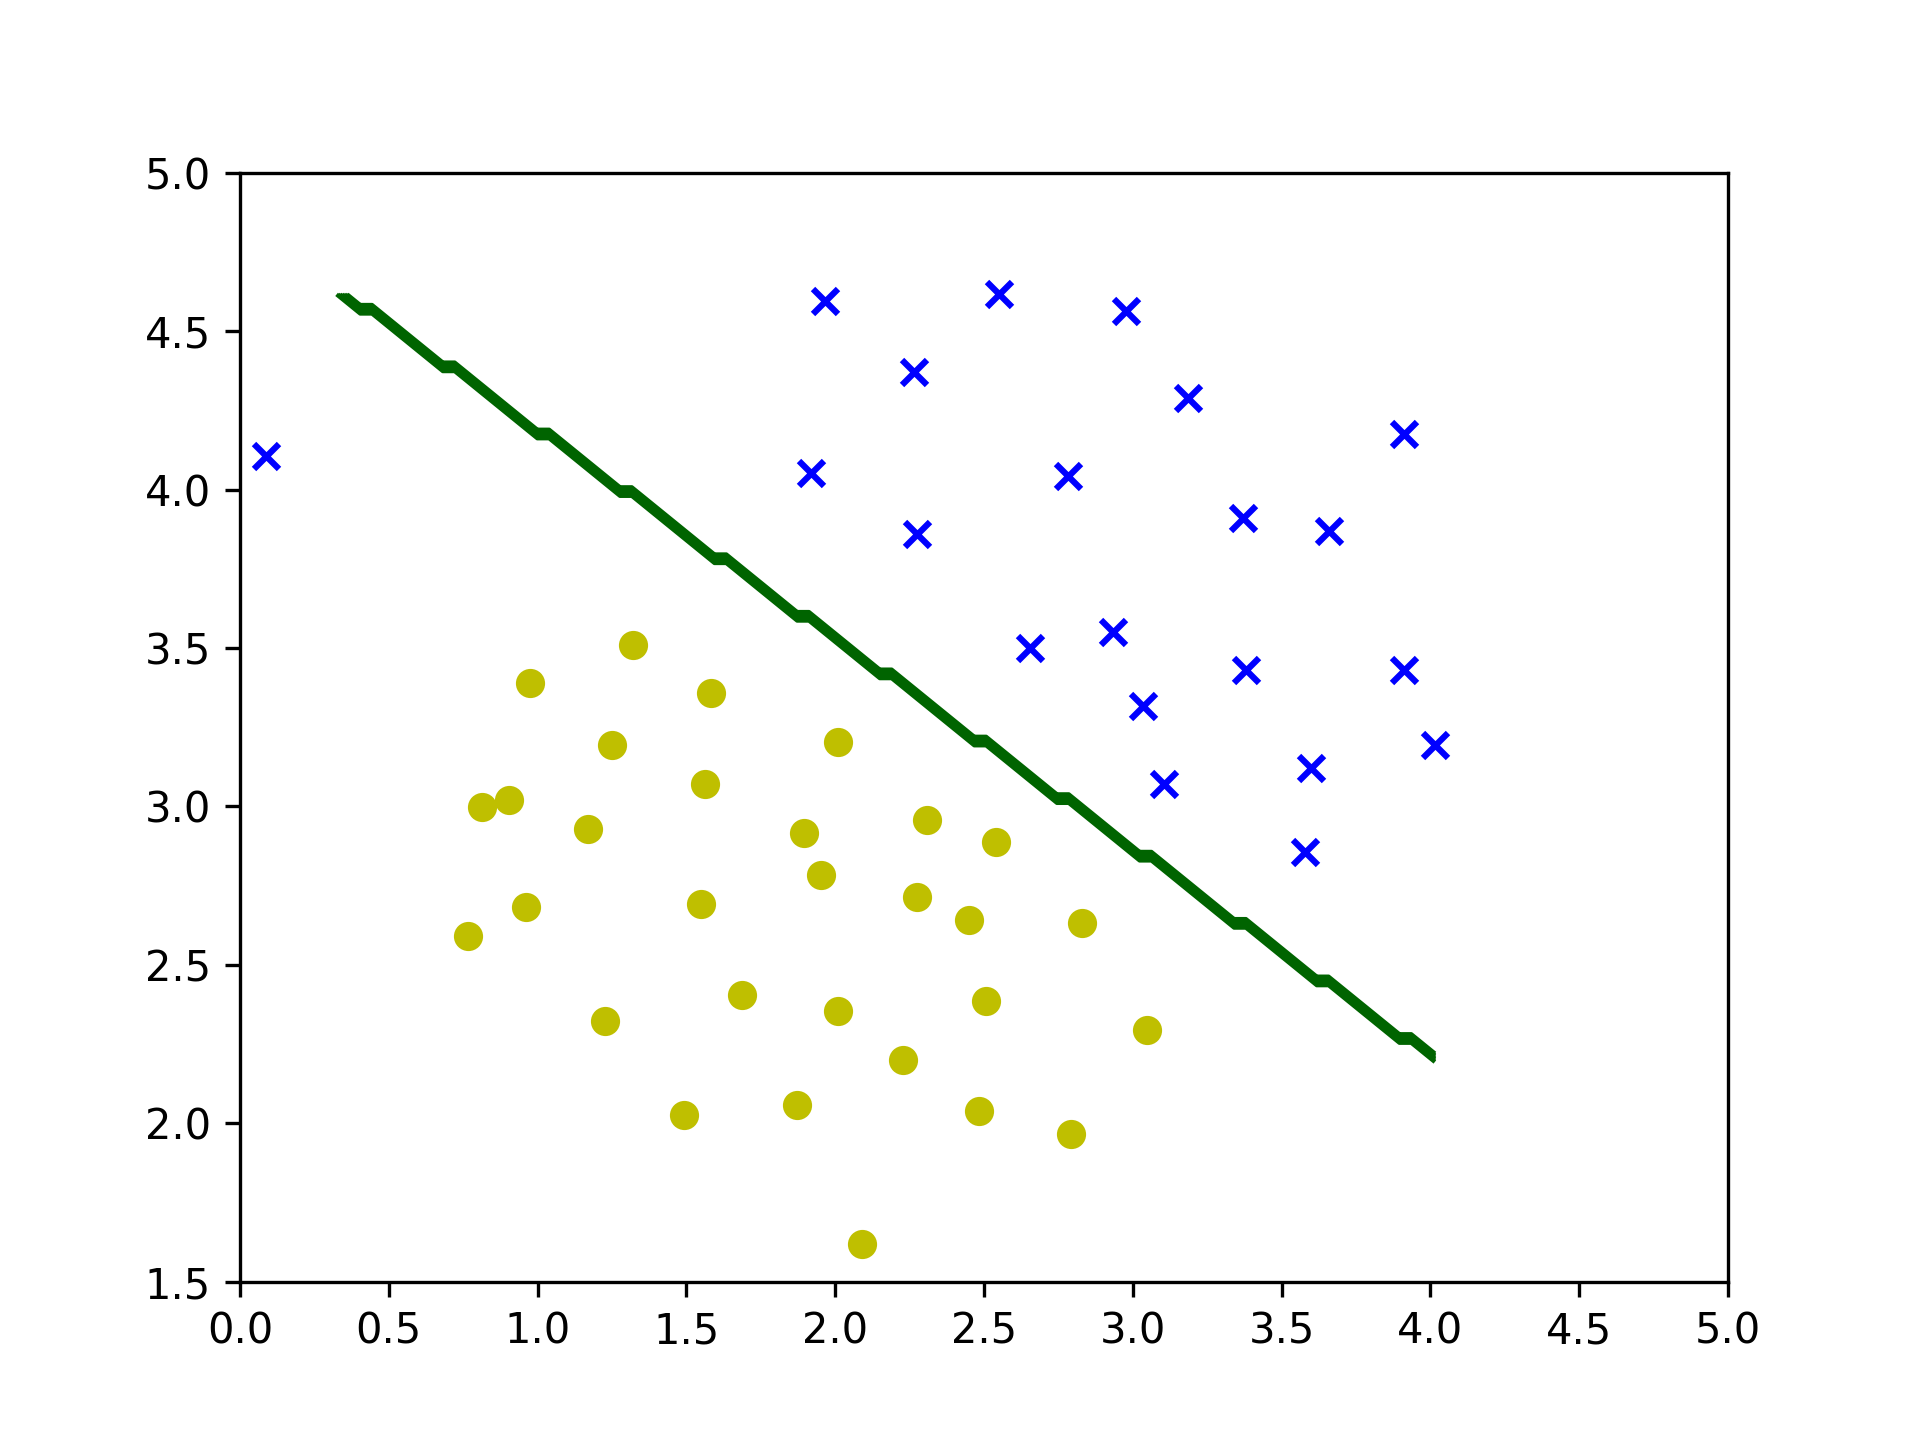
\includegraphics[width=0.8\textwidth]{./images/SVM_lineal_c1.0.png}
    \caption{SVM lineal con C=1.0}
\end{figure}

\begin{figure}[H]
    \centering
    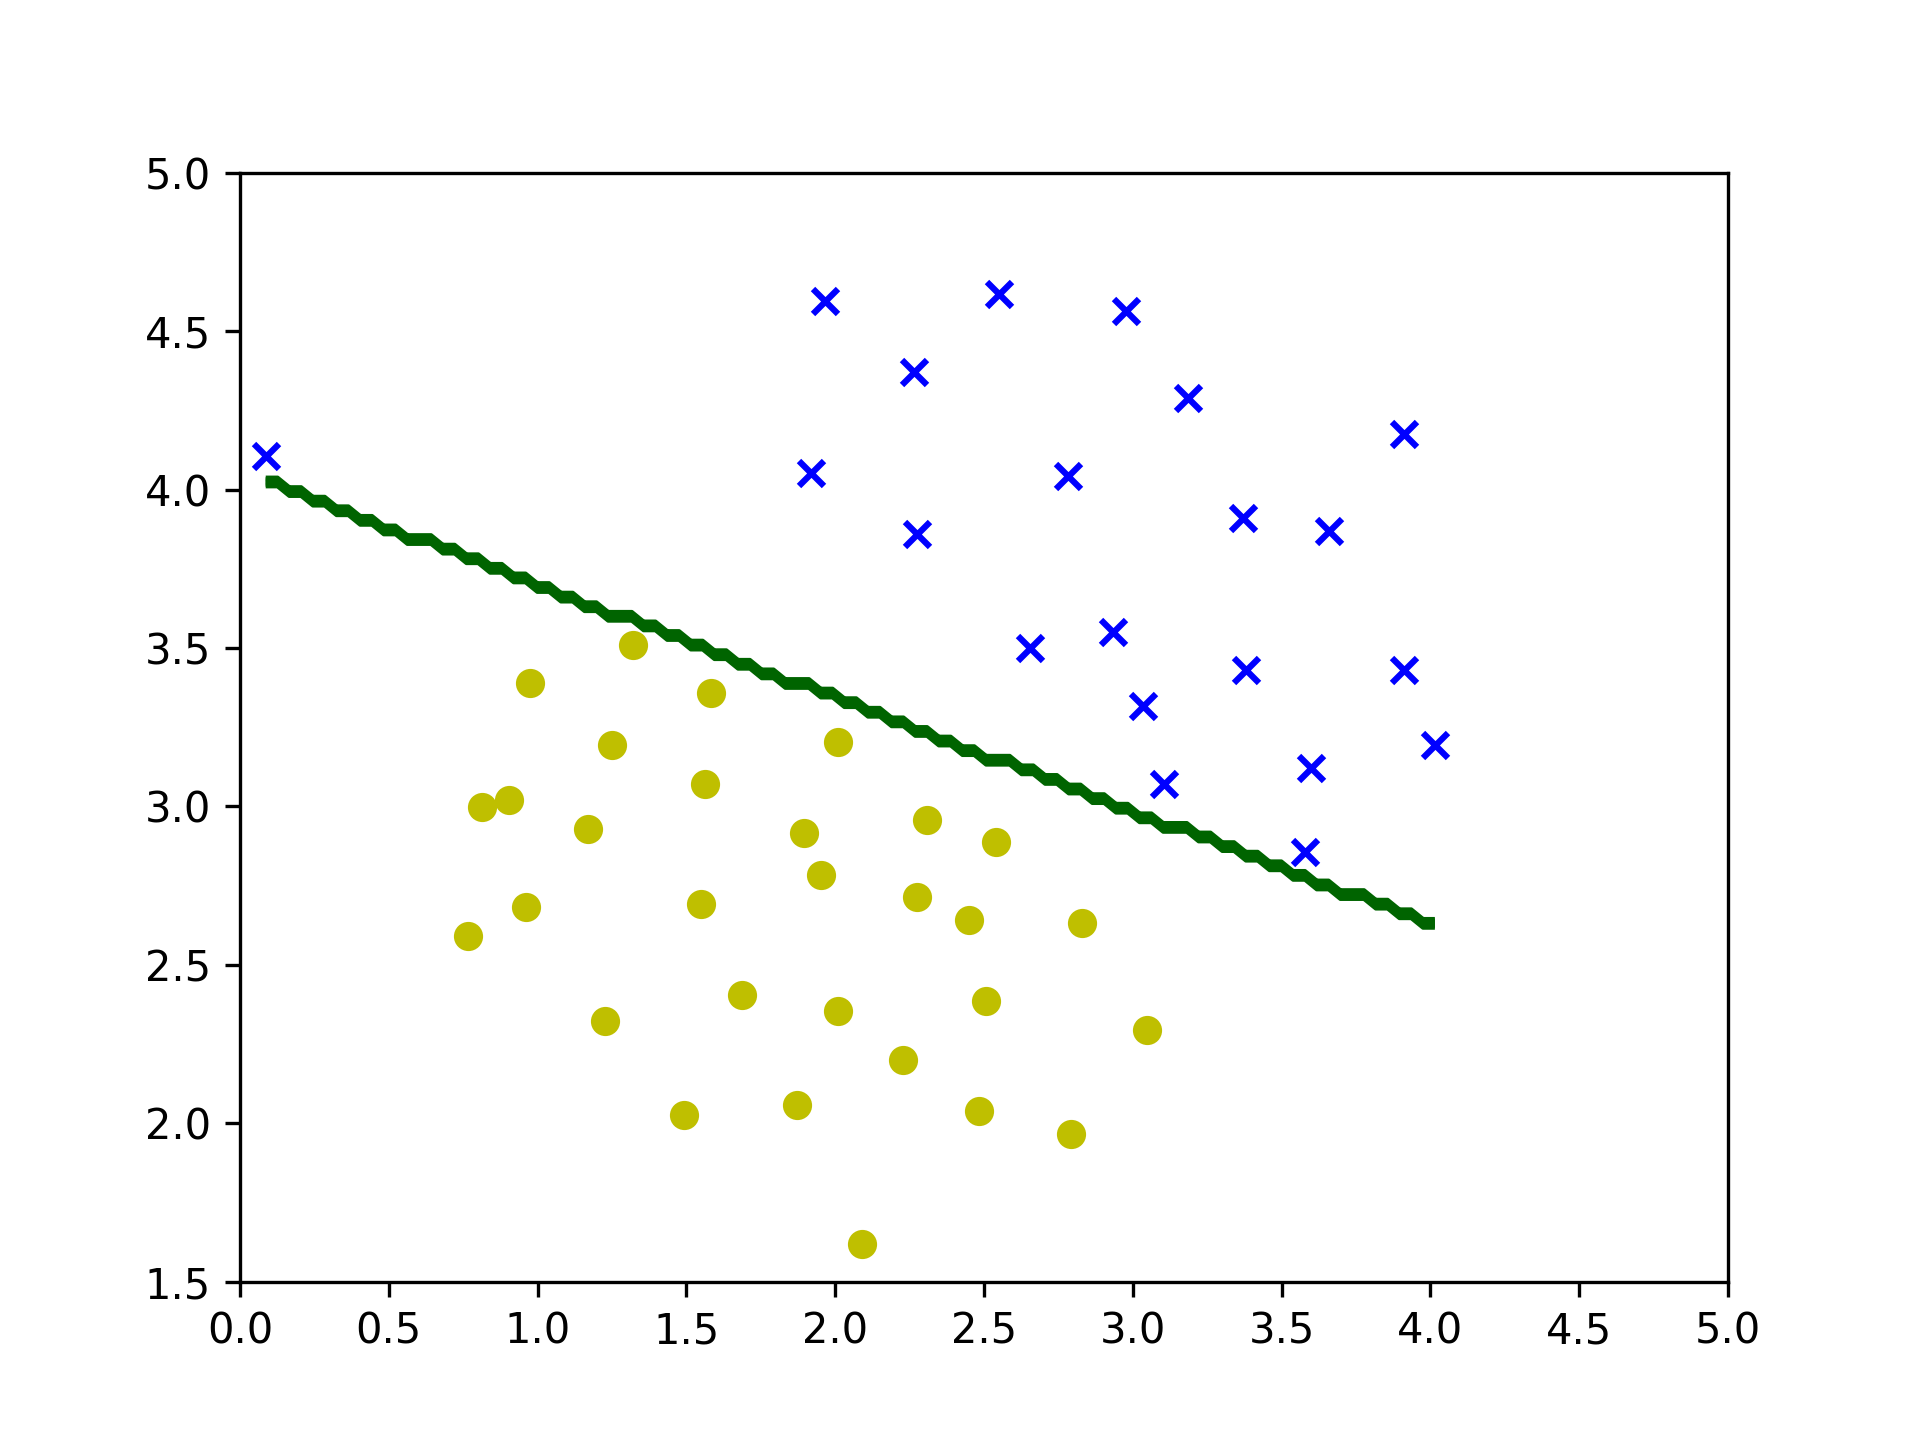
\includegraphics[width=0.8\textwidth]{./images/SVM_lineal_c100.0.png}
    \caption{SVM lineal con C=100.0}
\end{figure}

\begin{figure}[H]
    \centering
    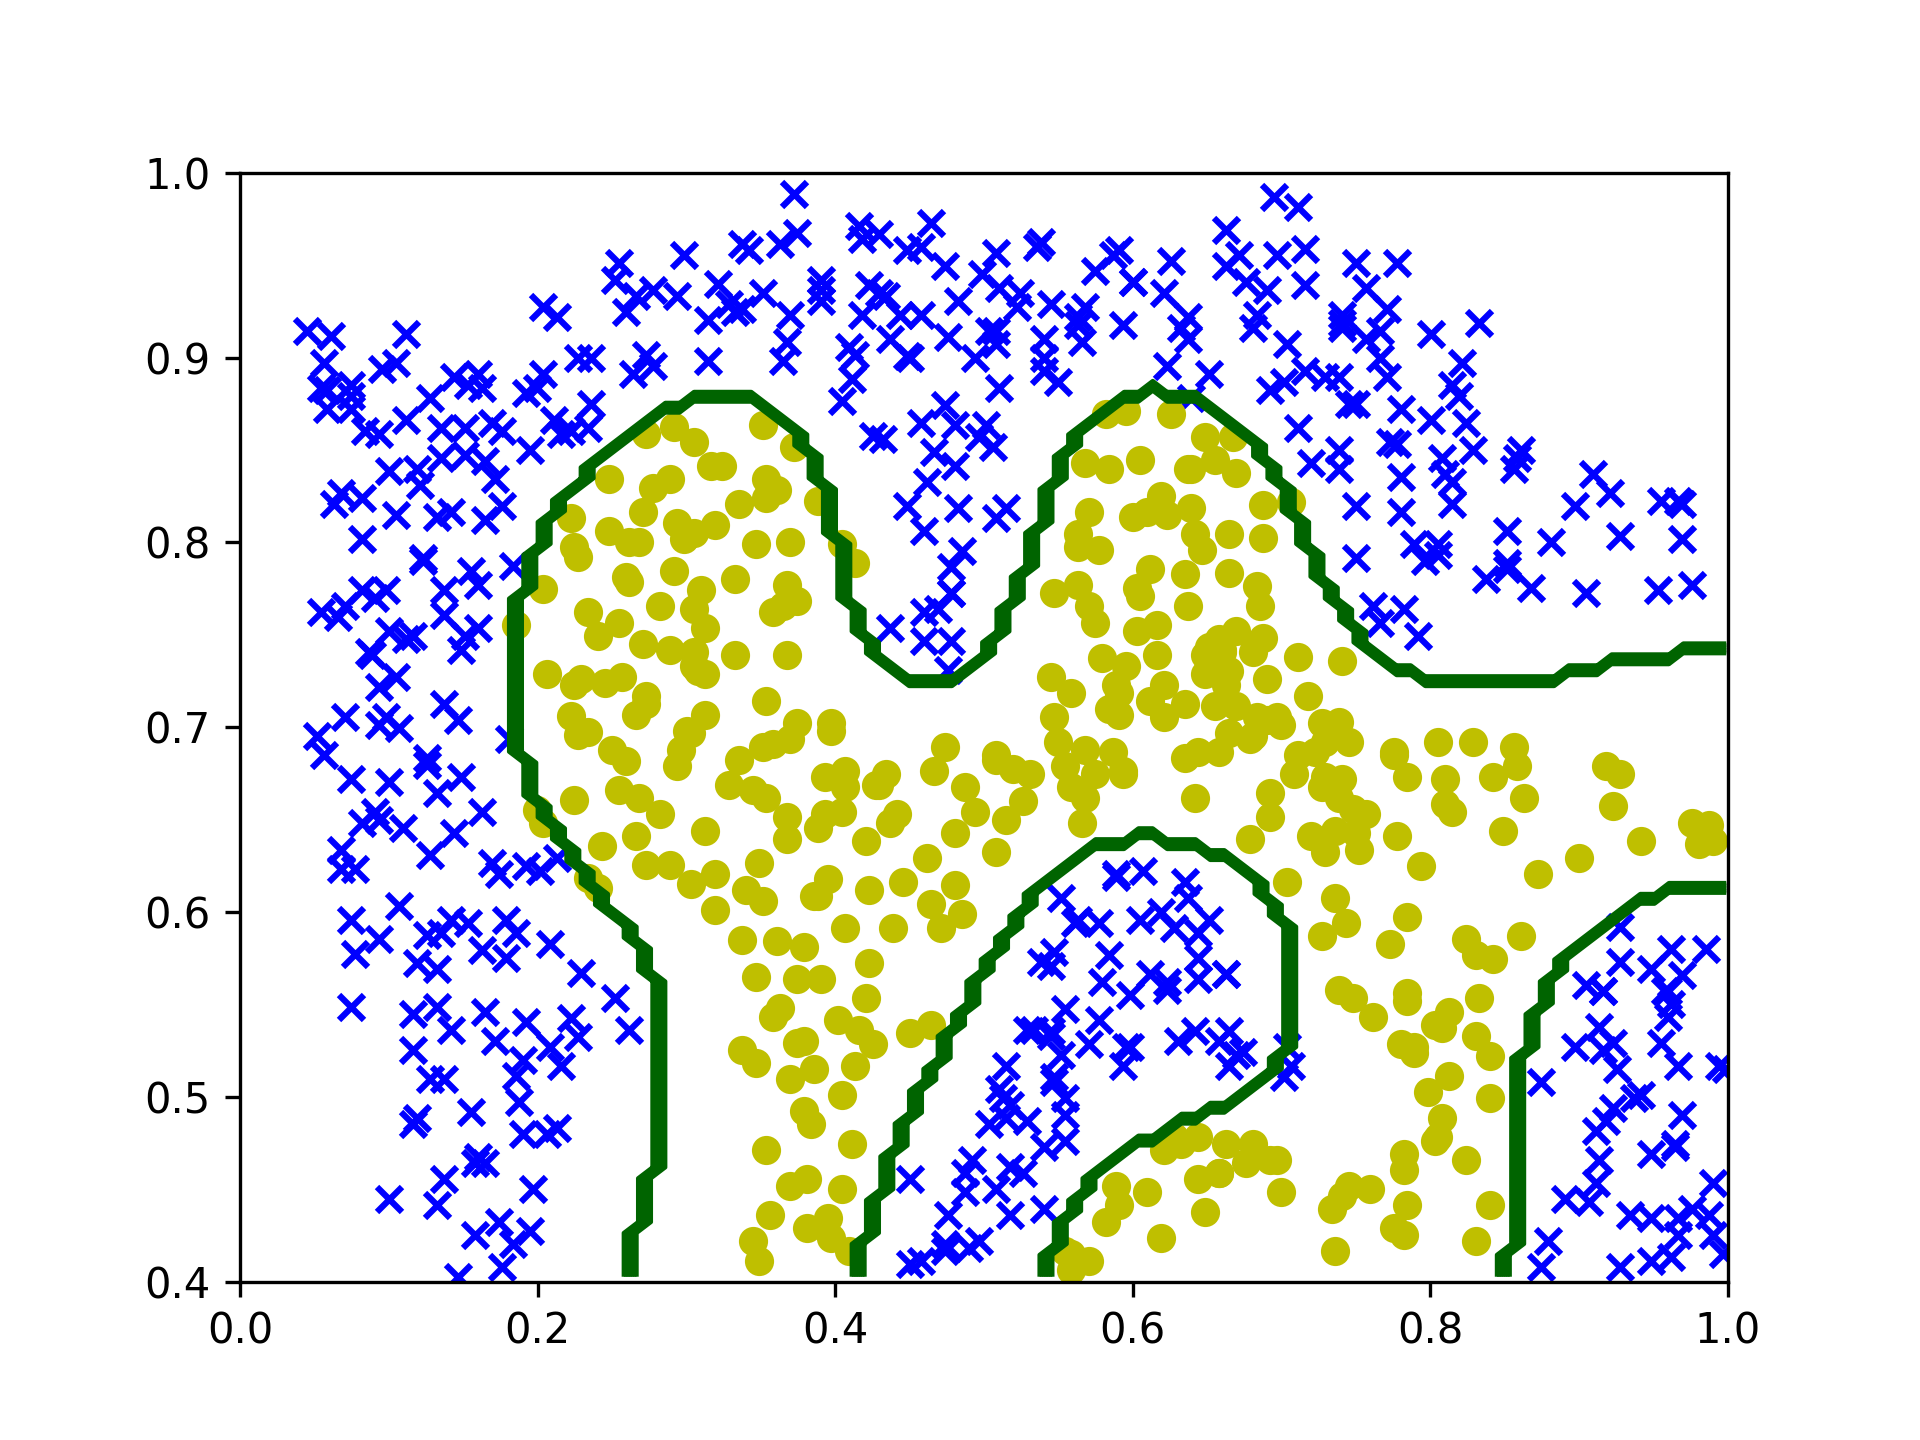
\includegraphics[width=0.8\textwidth]{./images/SVM_gauss_c1.0_sigma0.1.png}
    \caption{SVM gaussiano con C=1.0 y sigma=0.1}
\end{figure}

\begin{figure}[H]
    \centering
    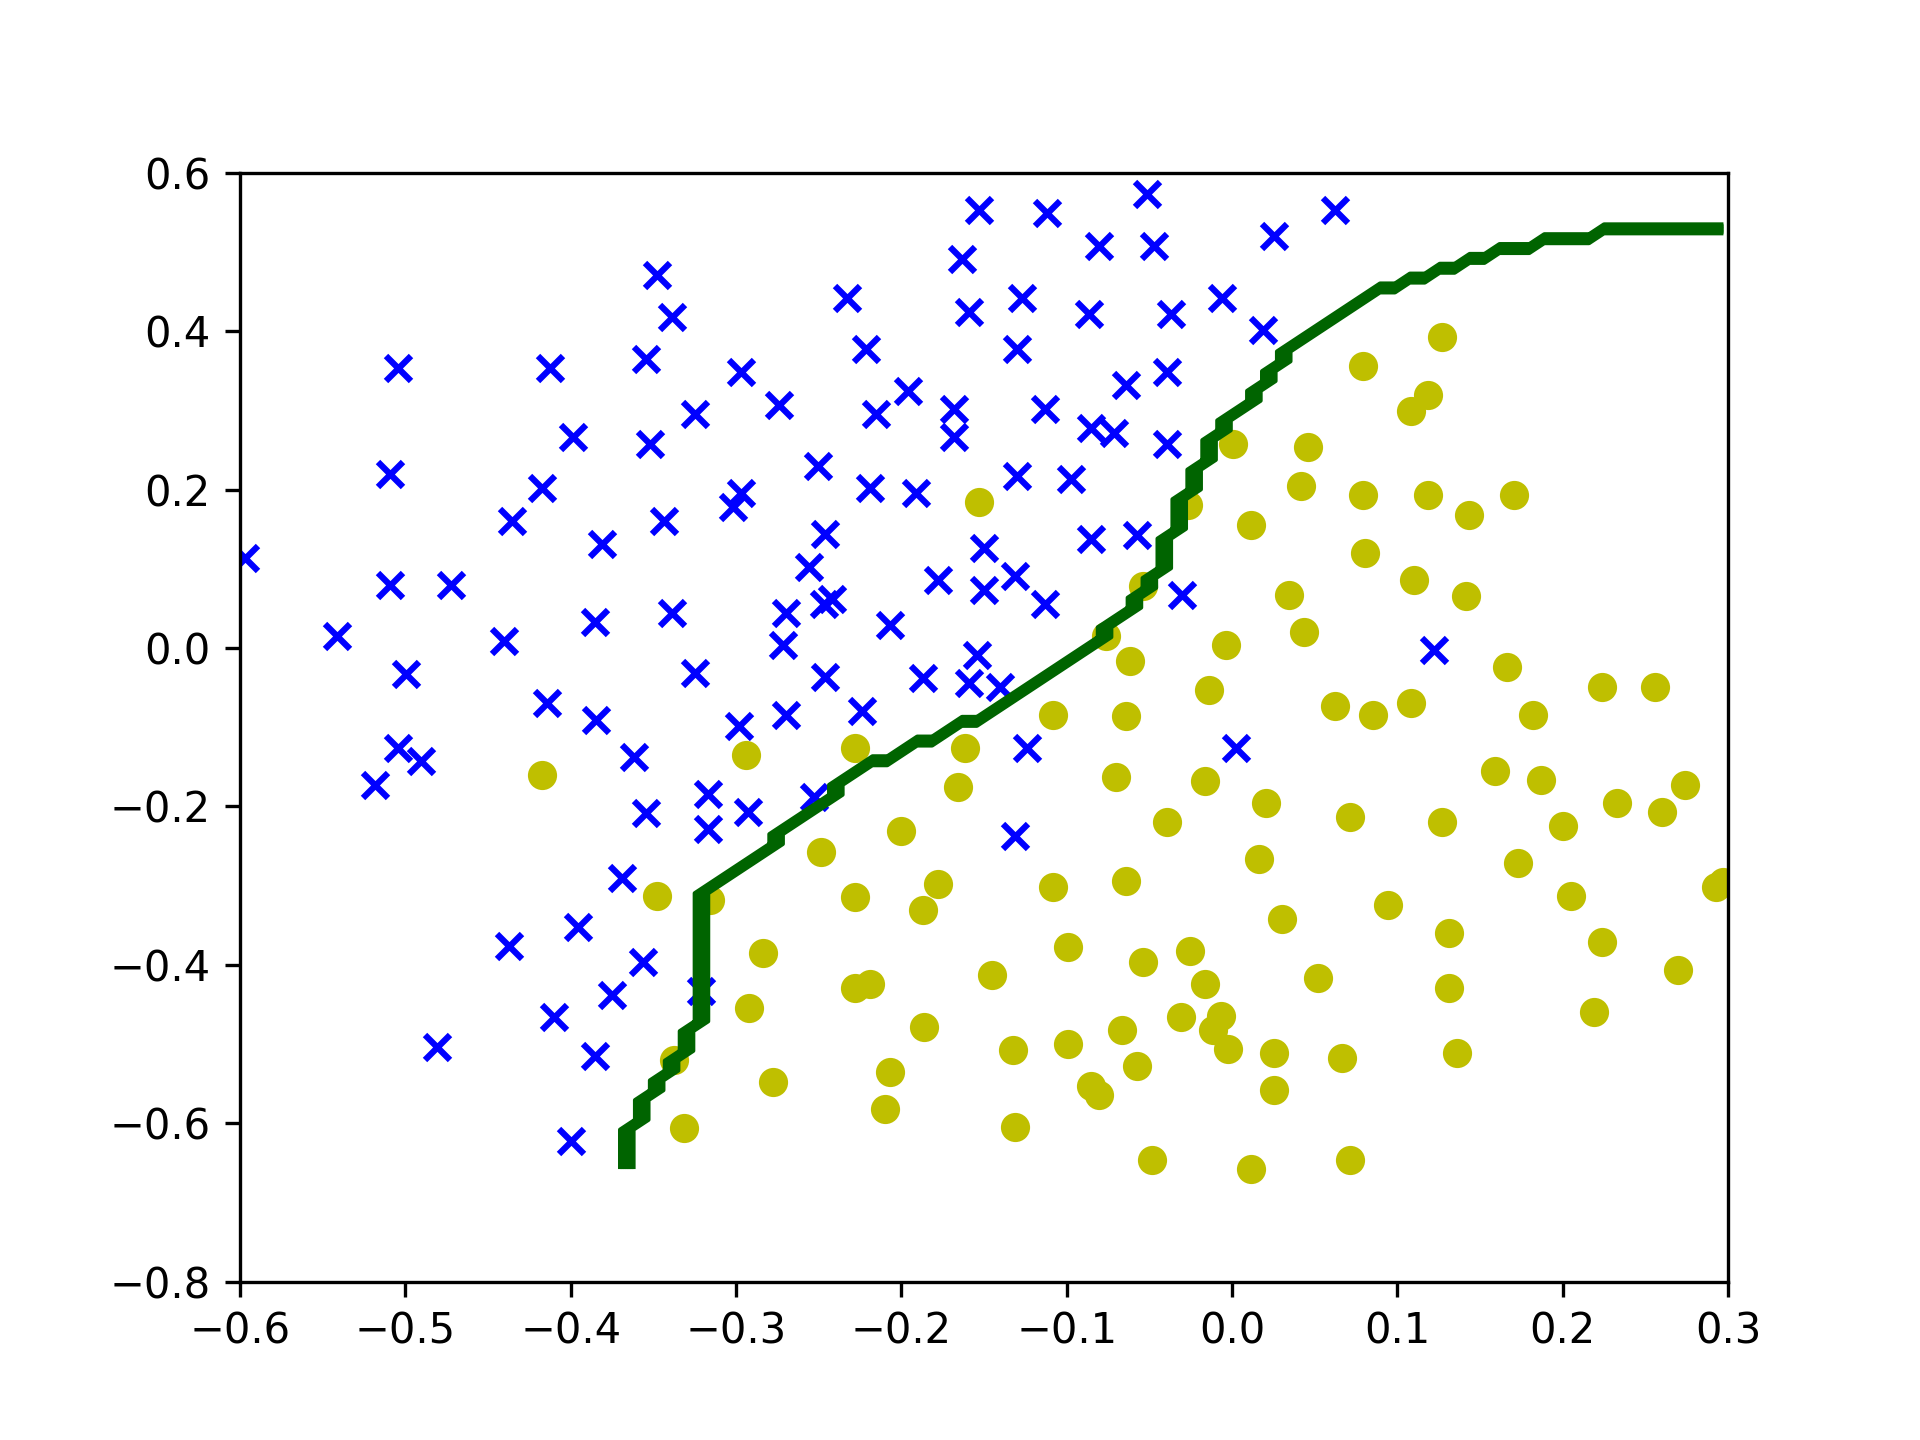
\includegraphics[width=0.8\textwidth]{./images/SVM_gauss_best.png}
    \caption{SVM gaussiano con C=1.0 y sigma=0.1, mejor configuración  para este problema}
\end{figure}

\section{Apartado B}

Para este problema usaremos distintos modelos:
\begin{itemize}
    \item \textbf{Regresión  lógica:} parece que  sobreentrena en train, tiene  como  resultados 100, 97, 98 en train, validación y test respectivamente. Tarda 7.73 segundos en su mejor modelo  con parámetros (10,  0.1)
    \item \textbf{SVM gaussiano:} mejor  modelo de todos, tiene 98, 97, 98 en train, validación y test respectivamente. Tarda  1 segundos en su mejor modelo con parámetros (1.0, 10.)
    \item \textbf{NN:} el modelo que más tarda de todos (posiblemente porque  está implementado en python  a mano y no con una biblioteca hecha en  un lenguaje competente) con resultados 96,  96 y  95 en train, validación y test respectivamente. Tarda  214 segundos en su mejor modelo con parámetros (3, 30)
    \item \textbf{Pytorch:} modelo entrenado en GPU con resultados 97, 97, 96 en train, validación y test respectivamente. Tarda  33 segundos en su mejor modelo con parámetros (0.001, 0.01)
    \item \textbf{PolynomialTransformer:} inviable a partir de grado  1, crashea  el ordenador porque la matriz de datos  es demasiado  grande.
\end{itemize}

Código del entrenador de regresión lógica:
\lstinputlisting[style=custompython]{../Logic_Regression_Trainer.py}

Código del entrenador de SVM gaussiano:
\lstinputlisting[style=custompython]{../SVM_Trainer.py}

Código del entrenador de NN:
\lstinputlisting[style=custompython]{../nn_Trainer.py}

Código del entrenador de Pytorch:
\lstinputlisting[style=custompython]{../pytorch_Trainer.py}

Código del entrenador de PolynomialTransformer:
\lstinputlisting[style=custompython]{../Poly_Trainer.py}


\begin{figure}[H]
    \centering
    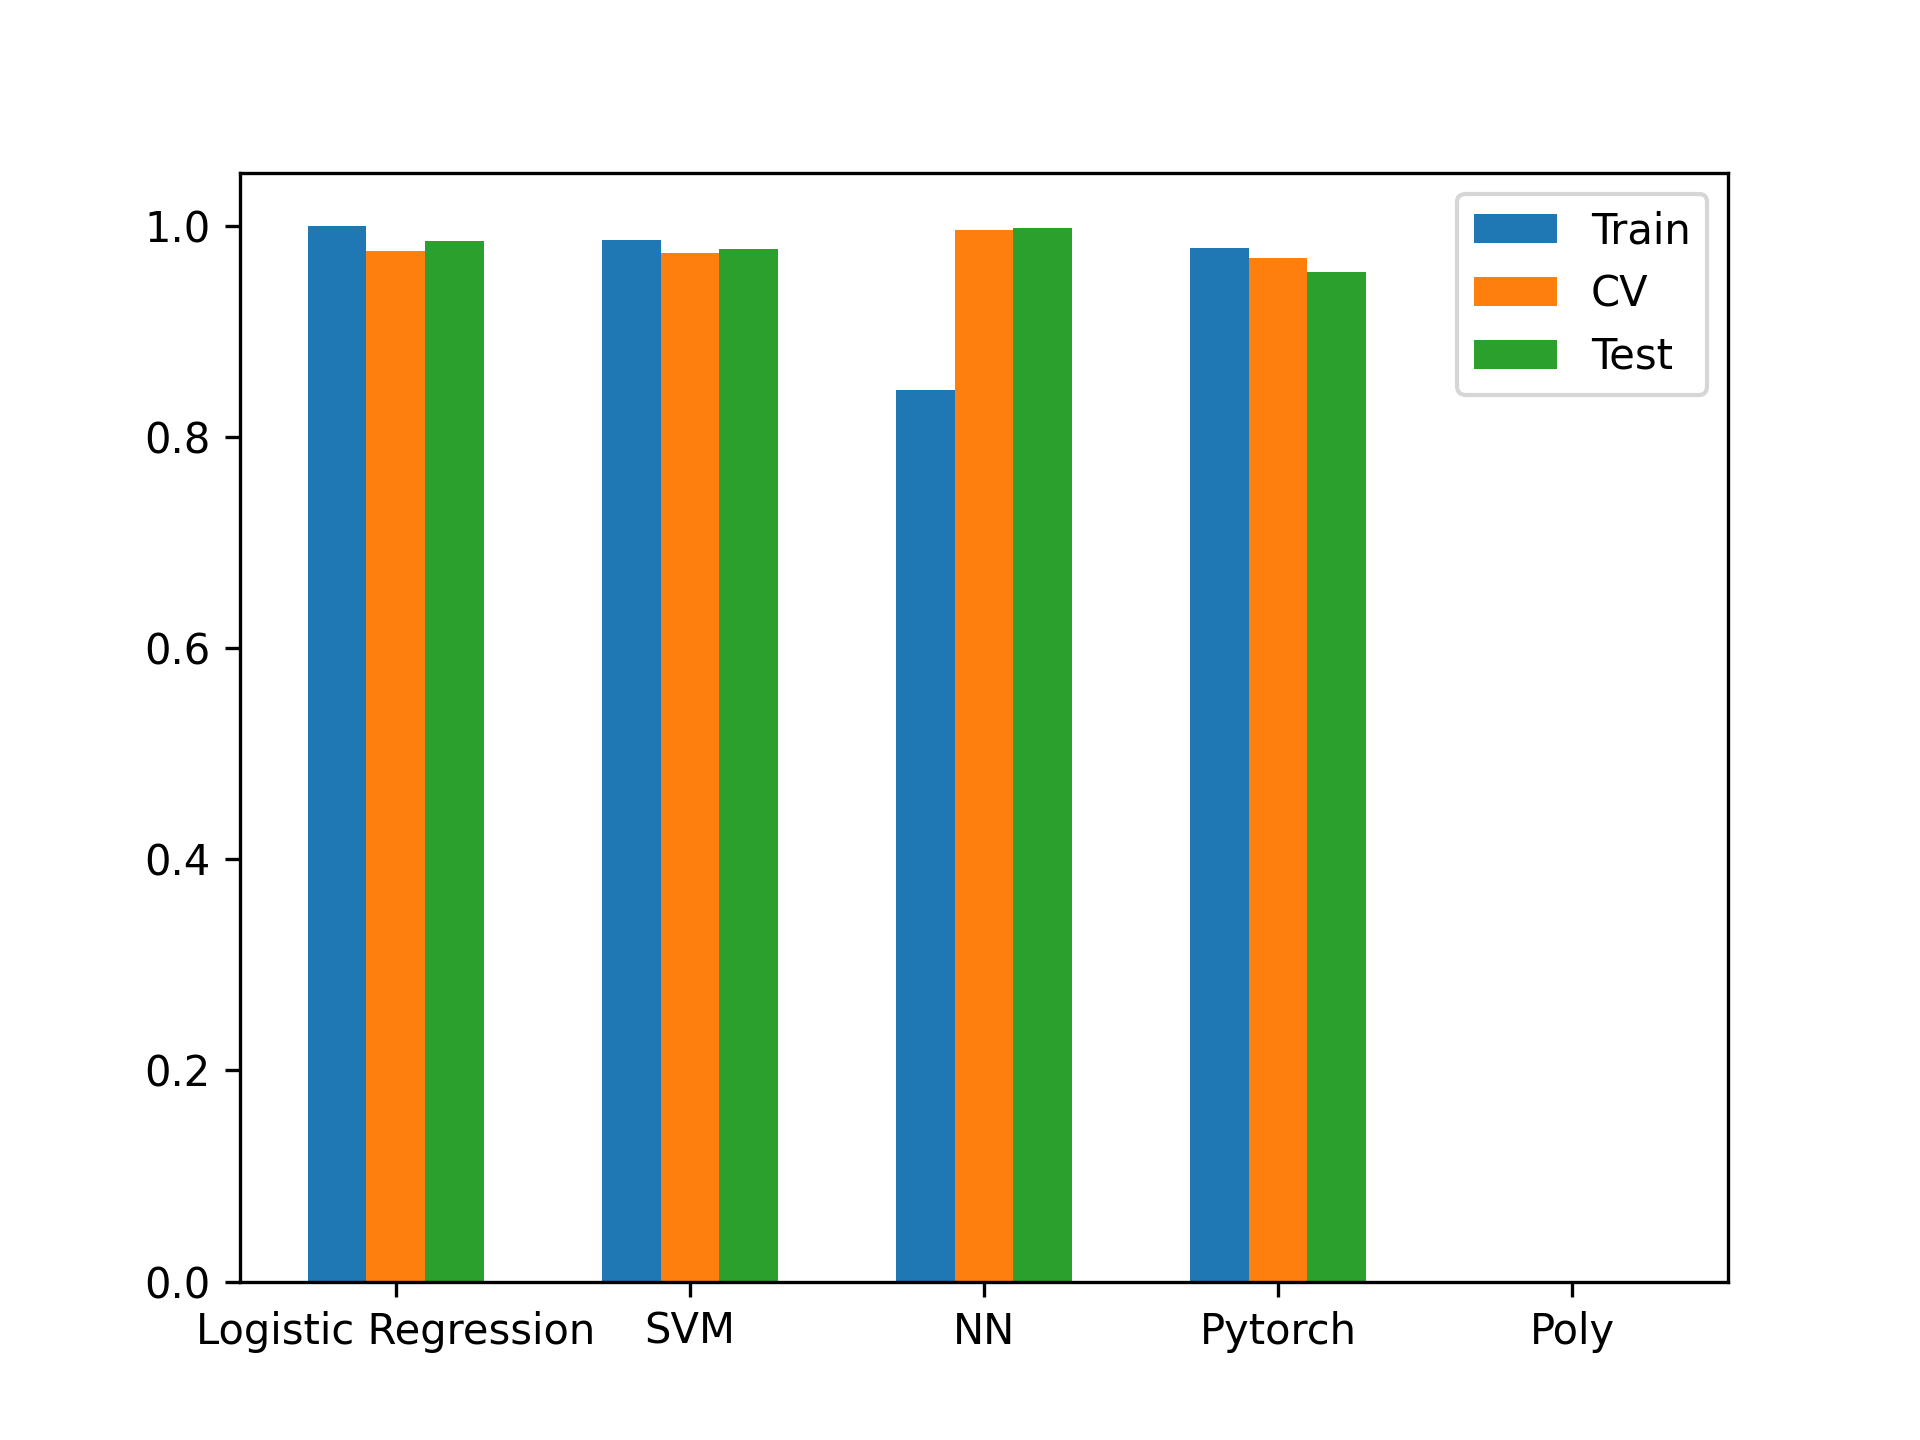
\includegraphics[width=0.8\textwidth]{./images/results.png}
    \caption{Resultados de los distintos modelos en precisión}
\end{figure}

\begin{figure}[H]
    \centering
    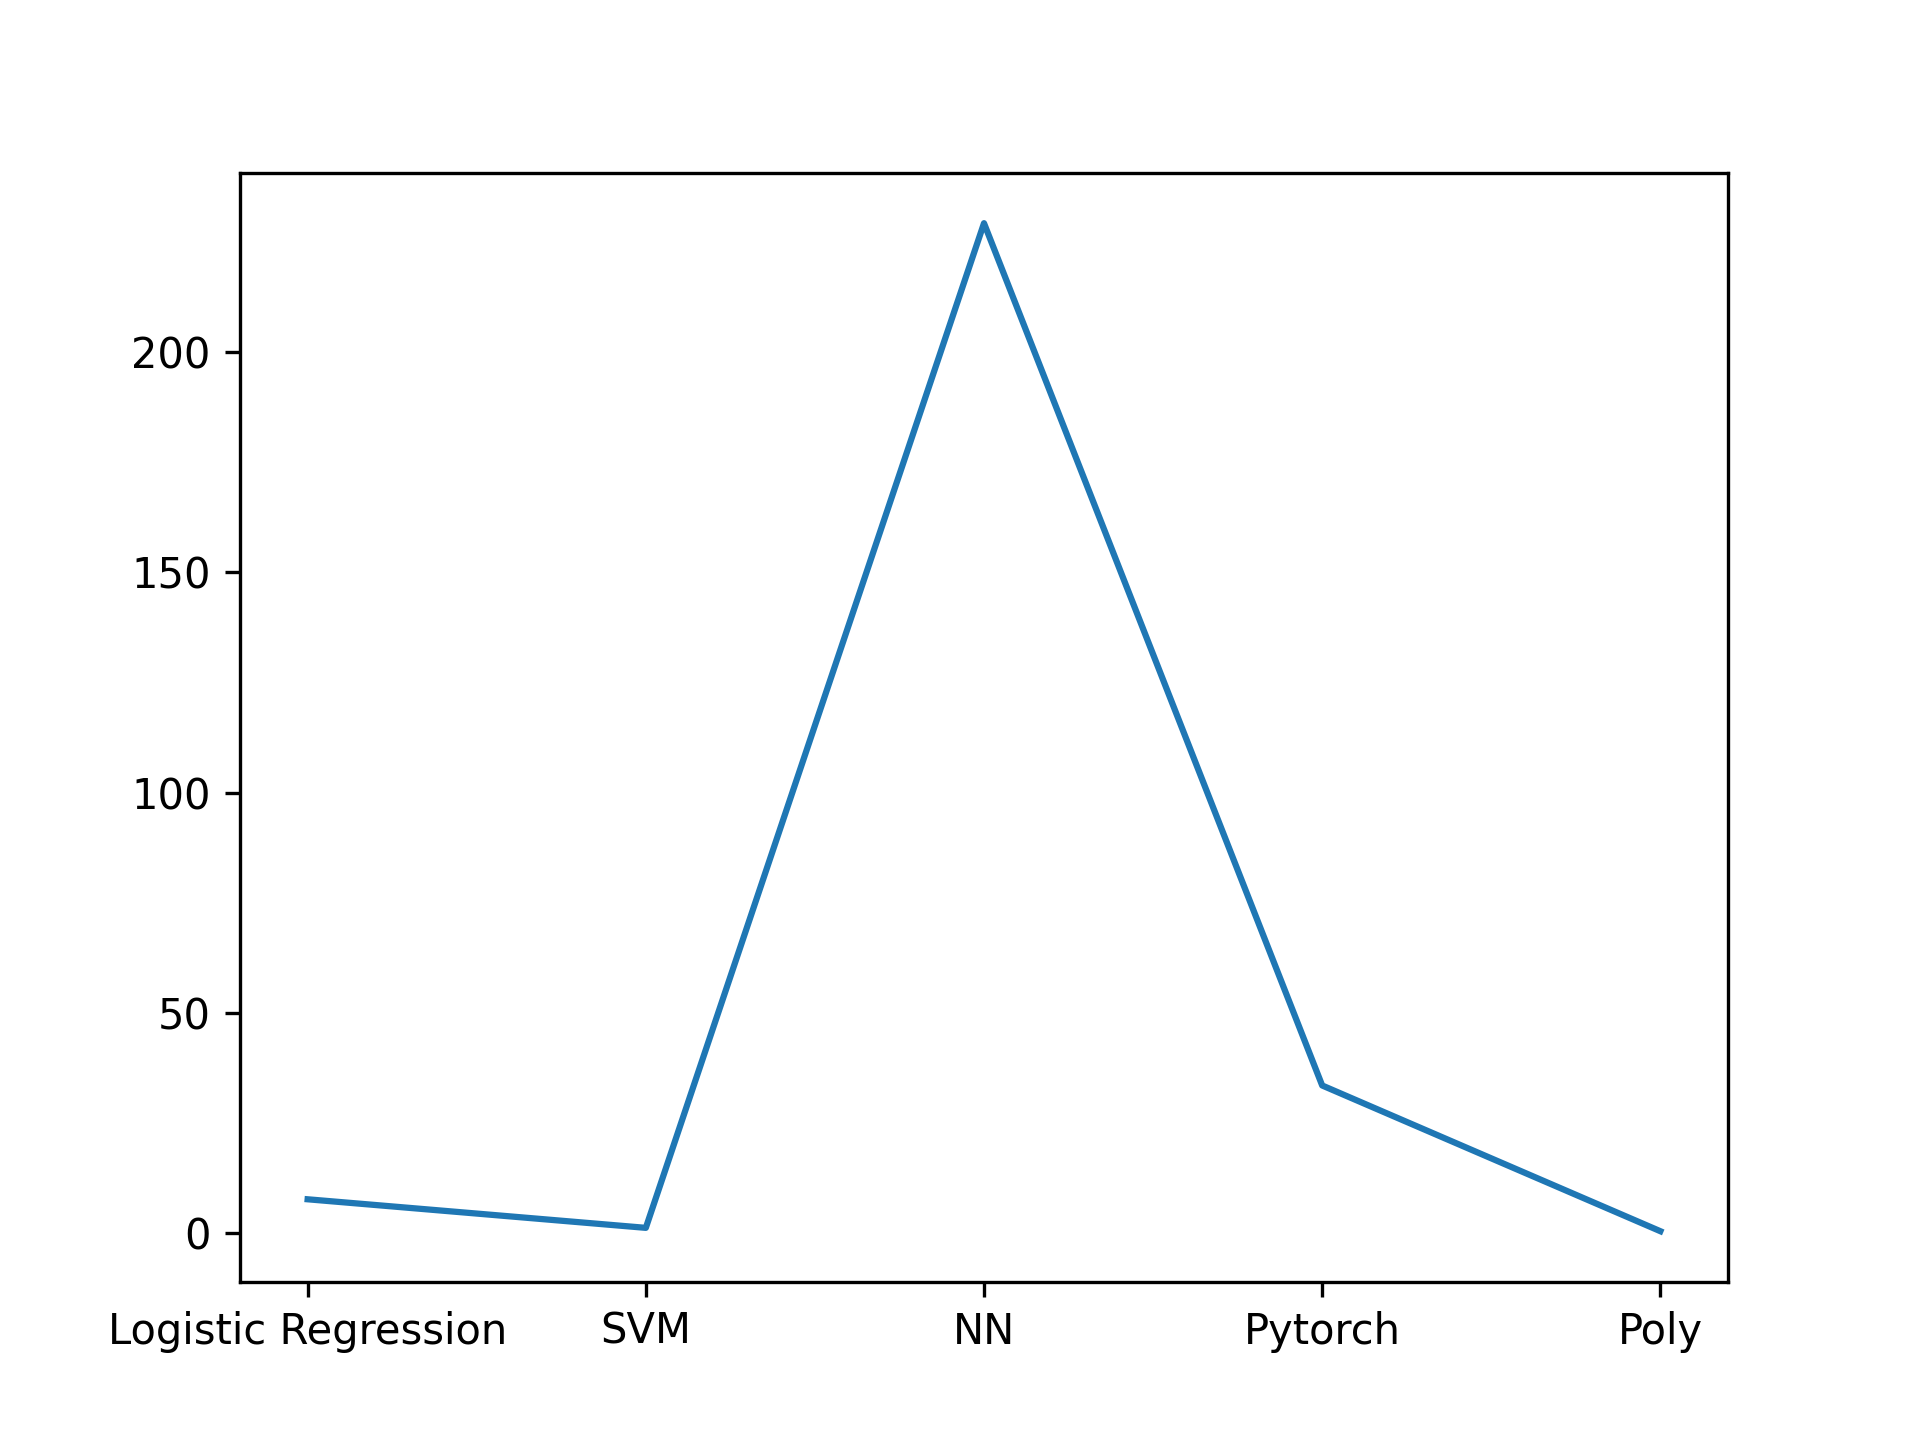
\includegraphics[width=0.8\textwidth]{./images/times.png}
    \caption{Tiempo de entrenamiento de los distintos modelos}
\end{figure}

\end{document}
